%!TEX root =  ../main.tex

\section{Number Line}\label{sec:NumberLine}

\objective{Solve absolute value linear equation and inequalities.}


\subsection{Negative Numbers}
As mentioned in the previous section, negative number arose as an extension of the whole 
numbers which accounted for all cases of subtraction.  What is the difference between
someone who has no money, and someone who owes \$3?  You can't tell until they are
paid \$3: one will have \$3 and the other will be broke!  

The imagery of debt brings in a helpful cognitive metaphor: quantities can have a direction, 
and not simply be a \gls{scalar}.  Once direction is involved, it is necessary to speak of 
opposites, which are easily framed as a positive and a negative frame of reference.  The
discovery of negative numbers recast what has simply been ``numbers'' as \emph{positive}
numbers.  In our system, positive is generally rightward, while negative is leftward.

\begin{example}
	\exProblem
What is five plus negative three?  What is five minus negative three?  Why?
	\exSolution
Suppose we are discussing money.  Someone having \$5 has added a debt of \$3 to his
or her ledger.  The net worth of such a person has decreased to \$2.  However, if someone
worth \$5 has a \$3 debt \emph{removed} from his or her account, the net worth of such a
person has increased (do to removed debt), and is now \$8.
\end{example}

\subsection{Absolute Value}
\index{Absolute Value!for distance}
After the introduction of directionality to numbers, it is often necessary to disregard such information.
Rather than caring about how far forward or backwards something has travelled, we only need to 
know the \emph{distance}.  The operation of ignoring the sign of a quantity is called the 
\emph{absolute value}.  Without other arguments, it answers the question, ``How far is a given
quantity from the center, from zero?''  For example, $|x-0| = 4$ is an algebraic way of asking for
the \emph{two} numbers four away from zero.  To include the subtraction operator, we should
really ask for the ``the two numbers who's difference with zero is four.''

\begin{example}
	\exProblem
What are the two numbers who's difference with negative seven is six?  How would one
represent this problem in algebra?
	\exSolution
If we travel six units to the right from negative seven, we arrive at negative one.  If we travel
six units to the left, negative thirteen.  This can be written as $|x-(-7)|=6$ or even better
$|x+7|=6 \therefore x=\{-13,-1\}$.
\end{example}

Looking only at the algebra, it can be beneficial to think of an absolute value sign in terms 
of the two cases it presents: a leftward possibility, and a rightward one.
Once an absolute value expression is reduced down to a simple equality, either the contents
of the absolute value is positive or negative.  For exampe, 

\begin{align*}
2|3x+1|+4=12\\
|3x+1|=4\\
3x+1=4 \\
\text{or}\\
3x+1=-4\\
x=\{1, -\frac{5}{3}\}
\end{align*}


\subsection{Inequalities}
\index{Absolute Value!inequalities}
Absolute value inequalities require logical reasoning, because if the distance to a given center
is \emph{less} than some number, the solution must be less than the center plus the distance
\emph{AND}  greater than the center minus the distance.  For example, $|x-117.5|<3.44$.

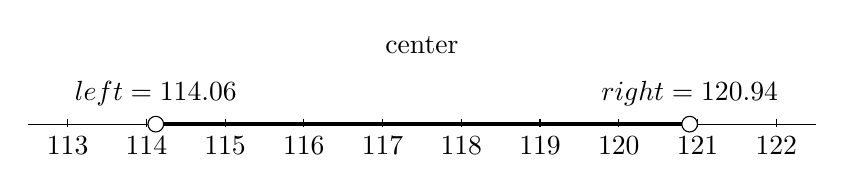
\begin{tikzpicture}
% a straight line segment
\draw (0.5,0) -- (10.5,0);
% the ticks and their labels
\foreach \x  in {1,...,10}
  \draw[xshift=\x cm] (0pt,2pt) -- (0pt,-1pt) node[below,fill=white] {\the\numexpr\x +112\relax};
% the thicker segment
\draw[ultra thick] (2.06,0) -- (8.94,0);
% the labels
\node[fill=white,draw=black,circle,inner sep=2pt,label=above:{$left=114.06$}] at (2.12,0) {};
\node[fill=white,draw=black,circle,inner sep=2pt,label=above:{$right=120.94$}] at (8.9,0) {};
\node at (5.5,1) {center};
\end{tikzpicture}

On the other hand, if the distance asked for this \emph{greater} than some number, the solution
must be more than the center plus the distance \emph{OR} less than the center minus the 
distance.  For example, $|x-117.5|\ge3.44$.

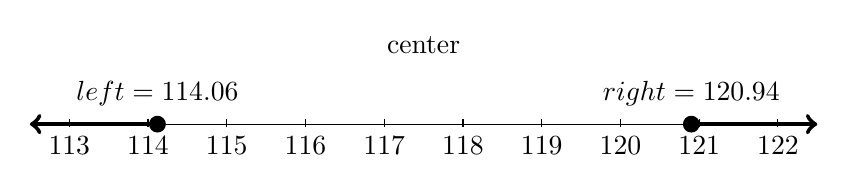
\begin{tikzpicture}
% a straight line segment
\draw (0.5,0) -- (10.5,0);
% the ticks and their labels
\foreach \x  in {1,...,10}
  \draw[xshift=\x cm] (0pt,2pt) -- (0pt,-1pt) node[below,fill=white] {\the\numexpr\x +112\relax};
% the thicker segments
\draw[ultra thick, ->] (2.06,0) -- (0.5,0);
\draw[ultra thick, ->] (8.94,0) -- (10.5,0);
% the labels
\node[fill=black,draw=black,circle,inner sep=2pt,label=above:{$left=114.06$}] at (2.12,0) {};
\node[fill=black,draw=black,circle,inner sep=2pt,label=above:{$right=120.94$}] at (8.9,0) {};
\node at (5.5,1) {center};
\end{tikzpicture}

Notice the convention is to indicate values which are attainable (``or equal to'') with solid
dots, while values not possible are marked as boundaries with hollow circles.

\ExSection[Exercises]
Graph on a number line

\begin{exercises}{sec:NumberLine}
\prob{}x < 2

\prob{}x <= 3

\prob{}x > 5 bowl x <=10

\prob{}|x| = 3

\prob{}|x| = -2

\prob{}|x-4| = 0

\prob{}|x - 4| = 2

\prob{}|x + 4| = 2

\prob{}|x| > 3

\prob{}|x-1| > 2

\prob{}4|x+2| < 8
\end{exercises}

